\chapter{数据管理}
\chapterauthors{Michael A. Kohn 和 Thomas B. Newman}
\sourcepage{592}
开展临床研究需要选择设计、界定目标人群、规定预测和结局变量。最后，大部分参与者和变量信息都会进入数据库，用于存储、更新、监测并整理为统计分析格式。数据库也可保存通话日志、访视安排和报销记录等行政数据。

许多临床试验，尤其为药物器械监管申请作准备者，把创建录入表、管理监测收集过程、整理提取分析资料的专家称为\term{临床数据管理员}（clinical data managers）（1）。药企投入大量资源和人员；初学者即使规模小，也需重视，因为结论取决于数据准确性、完整性与安全性。单表数据库可用电子表格或统计程序；复杂数据库则需管理软件定义表、开发录入系统并监测资料。

\section{数据表}
所有计算机数据库均由数据表构成，行对应记录（参与者、事件或交易等），列对应字段（记录属性）。最简单的研究表，每行一名参与者，每列为姓名、出生日期、性别或结局等属性。
\sourcepage{593}
首列通常是唯一识别号，如 ParticipantID。依次分配1、2、3等无内在含义的整数，便于保密。

图19.1是假想的新生儿胆红素与5岁智商队列（受真实研究启发（2））的简化表。二分类预测变量 Hyperbili\_ind 表示有无高胆红素血症，连续结局 IQ 是5岁智商。这样的单一二维表易用电子表格或统计包处理，常称\term{平面文件}（flat file）。

\begin{figure}[htbp]\centering
\begingroup\fontsize{9.5}{13}\selectfont\setlength{\tabcolsep}{4pt}
\begin{tabular}{rllccrrrr}\toprule
ParticipantID & FName & DOB & Sex & Hyperbili\_ind & ExDate & ExWght & ExHght & IQ\\\midrule
2101&Robert&1/6/2010&M&1&1/29/2015&23.9&118&104\\
2322&Helen&1/6/2010&F&0&1/29/2015&18.3&109&94\\
2376&Amy&1/13/2010&F&1&3/22/2015&18.5&117&85\\
2390&Alejandro&1/14/2010&M&0&&&&\\
2497&Isiah&1/18/2010&M&0&2/18/2015&20.5&121&74\\
2569&Joshua&1/23/2010&M&1&2/13/2015&24.8&113&115\\
2819&Ryan&1/26/2010&M&0&&&&\\
3019&Morgan&1/29/2010&F&0&2/9/2015&19.1&105&105\\
3031&Cody&2/15/2010&M&0&4/16/2015&15.2&107&132\\
3290&Amy&2/16/2010&F&1&4/12/2015&18.0&102&125\\
3374&Zachary&2/21/2010&M&1&&&&\\
3625&David&2/22/2010&M&1&2/10/2015&19.2&114&134\\
3901&Jackson&2/28/2010&M&0&&&&\\\bottomrule
\end{tabular}\endgroup
\caption{新生儿高胆红素与5岁智商研究的“数据表视图”。Hyperbili\_ind 指出生后10天内总胆红素是否达到25 mg/dL；IQ 为5岁智商。2390、2819、3374、3901未接受5岁检查。FName＝名，DOB＝出生日期，Sex＝性别，ExDate＝检查日期，ExWght＝体重，ExHght＝身高。}
\end{figure}

\textbf{若每人有多次化验、用药或重复测量，单表便不足，}需用管理软件把重复测量存在独立表中（3，4）。每行一项测量，包括内容、日期时间及结果，并用参与者识别号连接原表。
\sourcepage{594}
这种\term{关系数据库}（relational database）中，一人可有多测量，称\term{一对多}（one-to-many）关系。每个测量表首列应是唯一记录号，即\term{主键}（primary key）；图19.2中为 ExamID。

\begin{figure}[htbp]\centering
% Original database screenshot, unchanged, source PDF p594; identifiers remain literal.
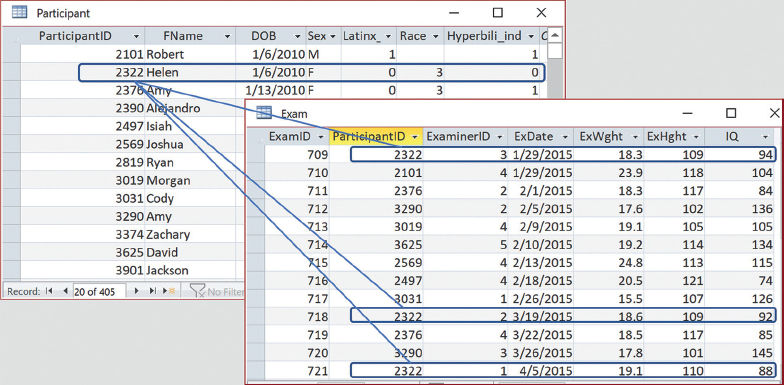
\includegraphics[width=\linewidth]{assets/ch19_fig02.png}
\caption{婴儿黄疸研究的双表数据库：Participant 每行一人，Exam 每行一次检查。2322号 Helen，出生日期1/6/2010，在下方不含姓名的表中有三次检查；蓝线连接这三行。ExWght 与 ExHght 存于检查表，不在参与者表。保留原软件中的字段名：ExamID＝检查号，ParticipantID＝参与者号，ExaminerID＝检查者号，ExDate＝日期，ExWght＝体重，ExHght＝身高，IQ＝智商。}
\end{figure}

虽然每人只有一次智商检查，但多数另有身高、体重等检查，可计算体质指数（BMI）和生长曲线百分位（见下文“提取数据〔查询〕”）。
\sourcepage{595}
宜单独建 Exam 表，一行一次检查，列包括日期、结果和参与者号。一人可多次检查，故为一对多。把检查资料连回个人资料的字段称\term{外键}（foreign key），此处为 ParticipantID。

双表结构中，查某时段全部检查只需搜索一个日期列；改变出生日期等个人字段只改一处，保持一致。姓名、生日等只在参与者表出现，检查表用 ID 连接；没有检查的 Alejandro、Ryan、Zachary、Jackson 也可保留。

详细化验需另一表。例如，记录出生后完整胆红素轨迹时，一行一结果，含日期时间、检验类型、结果及 ParticipantID 外键（图19.3）。
\sourcepage{596}
\begin{figure}[htbp]\centering
% Original database screenshot, unchanged, source PDF p596.
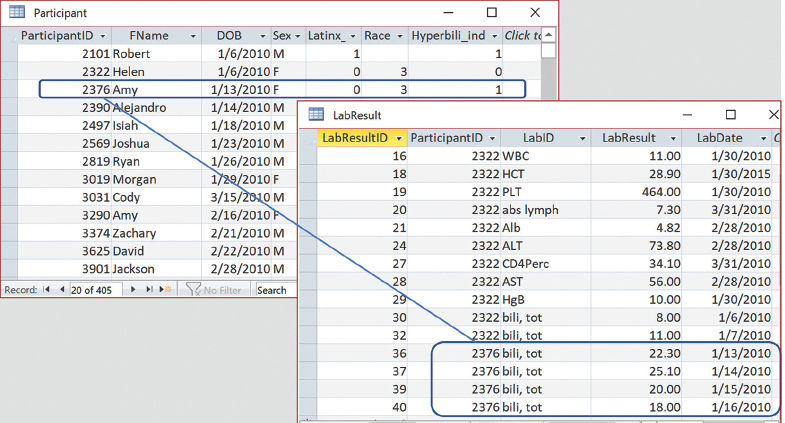
\includegraphics[width=\linewidth]{assets/ch19_fig03.png}
\caption{参与者表与化验结果表的连接。蓝线把 Amy（2376）连接至出生后前4天总胆红素：1/13/2010为22.30，1/14为25.10，1/15为20.00，1/16为18.00。LabResultID＝结果记录号，LabID＝检验项目，LabResult＝结果，LabDate＝日期；bili, tot 为总胆红素。原字段名及其他行的数据保留于软件画面中。}
\end{figure}

\textbf{行政资料也需独立表。}例如，有些家庭只打几次电话，难联系者可能50次以上。若每人一行，就需为最多通话数设足够多列，而多数为空；每次通话一行，以 ParticipantID 连接，容易得多。

把生日、出生体重、出生指定性别等每人单值字段放一表，把电话、胆红素等每人数量不定的多值字段放另一表，是\term{数据库规范化}（database normalization）的一部分。新表唯一的参与者特异字段应为 ParticipantID，其余个人字段仅存于每人一行的表。
\sourcepage{597}
规范化消除冗余与不一致机会。软件可维护\term{参照完整性}（referential integrity），不允许为未登记者建立检查、化验或电话记录，也不允许在未删除全部相关记录前删除该参与者。

\subsection{数据字典、类型和值域}
每一列或字段都必须有名称、数据类型和定义。例如，图19.2参与者表中的 FName 是保存参与者名字的文本字段，DOB 是保存出生日期的日期字段，Hyperbili\_ind 是说明胆红素是否超过25 mg/dL的是／否字段。检查表中的 ExWght 是以千克记录体重的连续数值字段，IQ 则是保存智商得分的离散整数字段。每个字段的类型和定义都应在\term{数据字典}（data dictionary）中明确列出。数据字典提供的是数据库自身的信息，因而称为\term{元数据}（metadata）。

图19.4以表设计／字典视图展示，每行一个字段，列包括名称、类型、描述和允许范围。例如 Sex 只允许 M、F，IQ 只允许40--200的整数。\footnote{后文提出更具包容性的性别编码。}管理员常称验证规则为“编辑检查”（edit checks）（1），可减少录入错误。有些类型自带规则，例如日期自动拒绝4月31日。
\sourcepage{598}
\begin{figure}[htbp]\centering\small
\begin{tabularx}{\linewidth}{L{.23\linewidth}L{.18\linewidth}Y}\toprule
字段名 & 数据类型 & 描述／允许值\\\midrule
\multicolumn{3}{c}{Participant（参与者表）}\\
ParticipantID & 数字 & 唯一参与者识别号\\
FName & 短文本 & 名\\
DOB & 日期／时间 & 出生日期\\
Sex & 短文本 & 性别：M 或 F\\
Latinx\_ind & 数字 & 西班牙裔或拉丁裔\\
Race & 数字 & \\
Hyperbili\_ind & 数字 & 高胆红素：是或否\\\midrule
\multicolumn{3}{c}{Exam（检查表）}\\
ExamID & 数字 & 主键\\
ParticipantID & 数字 & 外键：参与者\\
ExaminerID & 数字 & 外键：检查者\\
ExDate & 日期／时间 & 检查日期\\
ExWght & 数字 & 体重，kg\\
ExHght & 数字 & 身高，cm\\
IQ & 数字 & 智商\\\bottomrule
\end{tabularx}
\par\smallskip\raggedright
Sex 的字段属性：长度1；验证规则为“M”或“F”；必填、允许零长度、索引及 Unicode 压缩均为“否”；IME 模式为“不控制”，句子模式“无”，文字常规对齐；格式、输入掩码、标题、默认值及验证文本为空。

IQ 的字段属性：长整型；小数位自动；默认值0；验证规则为40至200；必填及索引“否”，常规对齐；格式、输入掩码、标题及验证文本为空。

图中软件的帮助提示：字段名最多64个字符，可以包含空格；按 F1 键可获取字段名的帮助。
\caption{参与者表和检查表的数据字典视图。各变量有名称、数据类型、描述及允许值集合或值域。上表保留作为代码使用的字段名，类型、说明和属性译为中文。}
\end{figure}

\subsection{变量名称与编码惯例}
名称应短到便于输入，又足够自明；不用空格和特殊字符，可用 InterCaps、camelCase 或下划线分词。二分类指标按“是／存在”命名，如 EverSmoker\_ind，是为1、否为0；此时均值就是具有属性的比例。加后缀 \_ind 便于识别。多数软件另可设较长、易读的标签用于表格报告。
\sourcepage{599}
一种惯例以9或99表示“不知道、不适用、未回答”等，8或88表示“其他（注明）”。性别、族裔和种族常采用国家卫生统计中心方式（5），已纳入若干 EHR。性别标准代码为：0女性，1男性，4跨性别女性转男性，5跨性别男性转女性，8非二元，9未知。

族裔与种族采用两题：
\begin{studyquote}
问题1：你认为自己是西班牙裔／拉丁裔吗？\\
问题2：以下五种种族名称，哪种最适合描述你？\\
美国印第安人或阿拉斯加原住民；亚裔；黑人或非裔美国人；夏威夷原住民或其他太平洋岛民；白人。
\end{studyquote}
第二题可多选（图19.5），也可加“其他（含不止一种种族）”和“未知／未报告”，再限单选。
\begin{figure}[htbp]\centering
\begin{bookbox}{种族——请在所有适用项标记 X}
1\ $\mdlgwhtsquare$ 白人\qquad 4\ $\mdlgwhtsquare$ 夏威夷原住民或其他太平洋岛民\\
2\ $\mdlgwhtsquare$ 黑人或非裔美国人\\
3\ $\mdlgwhtsquare$ 亚裔\qquad 5\ $\mdlgwhtsquare$ 美国印第安人或阿拉斯加原住民
\end{bookbox}
\caption{国家卫生统计中心全国医院门诊医疗调查的种族编码（6）。}
\end{figure}
\sourcepage{600}
族裔字段 EthnLatino\_ind 允许0（非西班牙裔／拉丁裔）、1（是）、9（未知／拒绝回答）。Race 则为：1白人；2黑人或非裔美国人；3亚裔；4夏威夷原住民或其他太平洋岛民；5美国印第安人或阿拉斯加原住民；6其他（含多种）；7未知／未报告。

\subsection{共同数据要素}
美国国家神经疾病与卒中研究所（NINDS）（7）、国家癌症研究所（8）、FDA（9）、欧洲药品管理局，以及非政府非营利的临床数据交换标准协会（Clinical Data Interchange Standards Consortium，CDISC）（10）等，已开始开发共同数据要素。

统一记录结构、字段名与定义、类型格式及表格，可避免每项新研究重复建设，并支持跨研究分享合并。这需要共同字典和带说明的收集工具，鼓励特定领域研究者使用。

\section{数据录入}
无论几张表、使用何种软件，都需把数据填入。过去常用纸表，临床试验称\term{病例报告表}（case report form，CRF），再由人员转录入计算机，最好通过便捷且自动验证的屏幕表单。
\sourcepage{601}
\subsection{电子数据采集}
手写纸表日益少见。一般应主要用在线表单，临床试验称\term{电子病例报告表}（electronic case report form，eCRF），可在平板、手机或笔记本等无线设备录入。优点包括：
\begin{itemize}
\item 直接入表，无二次转录，消除该来源错误；
\item 可验证并即时反馈越界值；
\item 可设置跳题，如只有回答吸烟者才出现每天包数。
\end{itemize}
有时可收集后立即打印，由参与者核实；若审计需纸质原件，可作为源文件。互斥且穷尽的选项，常以下拉列表或选项组呈现（图19.6A、B），熟悉在线表单者一般都认识。
\sourcepage{602}
\begin{figure}[htbp]\centering\small
\begin{bookbox}{A\quad 下拉列表：折叠时与展开时}
你接种过 COVID-19 疫苗吗？\quad $\bullet$ 是\quad $\circ$ 否\qquad\textcolor{red}{*必填}\\
你首先接种的是哪种疫苗？\quad \fbox{Pfizer\quad$\downarrow$}\qquad\textcolor{red}{*必填}\\
请输入首剂日期：\quad\fbox{\hspace{2cm}}\quad 今天\quad 月-日-年\qquad\textcolor{red}{*必填}
\tcblower
同一下拉列表展开后的选项：\\
\fbox{\begin{minipage}{.52\linewidth}
\textbf{$\checkmark$ Pfizer}\\Moderna\\AstraZeneca\\Johnson \& Johnson\\其他（请注明）
\end{minipage}}
\end{bookbox}
\begin{bookbox}{B\quad 选项组}
你接种过 COVID-19 疫苗吗？\quad $\bullet$ 是\quad $\circ$ 否\qquad\textcolor{red}{*必填}\\
你首先接种的是哪种疫苗？\qquad\textcolor{red}{*必填}\\
$\bullet$ Pfizer\quad $\circ$ Moderna\quad $\circ$ AstraZeneca\\
$\circ$ Johnson \& Johnson\quad $\circ$ 其他（请注明）
\end{bookbox}
\caption{互斥、穷尽选项的录入格式。A的下拉列表节省屏幕空间，但打印作纸质收集时不能使用；B的选项组占空间较多，但可打印。原例的选中值均为 Pfizer。}
\end{figure}
互斥回答对应单一字段；“所有适用项”并不互斥，需要每种可能各一个是／否字段。惯例上，多选用方框，互斥单选用圆形按钮。
\sourcepage{603}
应避免“所有适用项”，最好强制每项是／否，否则未勾选不知是不适用还是未回答。

\subsection{导入测量与化验结果}
人口资料、化验、双能 X 线吸收测量（DEXA）和 Holter 动态心电等，通常已在医院 EHR 中数字化。应尽量直接导入，避免成本与转录错误。系统几乎都能输出逗号分隔值（csv）或固定列宽文本供导入。临床试验称这种批量上传为“非 CRF 数据”（1）。

\subsection{数据管理软件}
\term{后端}（back end）是数据表，\term{前端}（front end）或界面是录入、查看、编辑的在线表单。多表数据库需关系软件维护后端（表19.1）；若纸质收集，仍需转录在线表单。
\begin{bookbox}{表19.1\quad 研究数据管理常用软件示例}
\begin{description}[leftmargin=1em,style=nextline]
\item[电子表格]Microsoft Excel；Apple Numbers；Google Sheets\textsuperscript{a}；Apache OpenOffice Calc\textsuperscript{a}。
\item[统计分析]SAS（Statistical Analysis System）；SPSS（Statistical Package for the Social Sciences）；Stata；R\textsuperscript{a}。
\sourcepage{604}
\item[集成桌面数据库]Microsoft Access（仅 Windows）；Filemaker Pro。
\item[关系数据库]Oracle；SQL Server；MySQL\textsuperscript{a}；PostgreSQL\textsuperscript{a}。
\item[集成网络研究数据管理平台]REDCap（许多学术机构托管\textsuperscript{a}）；QuesGen（主要学术用途，供应商托管）；MediData RAVE（主要非学术企业，供应商托管）；Oracle InForm（非学术企业，公司托管）；Datalabs EDC（企业，供应商托管）；OnCore；OpenClinica；EpiInfo\textsuperscript{a}。
\item[在线调查]SurveyMonkey；Zoomerang；Qualtrics。
\end{description}
\small\textsuperscript{a}免费。
\end{bookbox}
如第17章所述，调查工具可发送电邮或放网站，提供多种格式、跳题、汇总、报告与导出。SAS 等统计包有录入模块；Access、Filemaker 等也有丰富的屏幕表单开发工具。

许多研究采用集成网络平台，如范德堡大学学术联盟专为临床研究开发的 REDCap（Research Electronic Data Capture）。
\sourcepage{605}
它可建立管理调查、录入表和数据库，许多学术机构研究者可使用，对初学者是很好的自行操作工具，也提供收集工具库。但定制及高级功能有限：数据库为单表，每列一字段、每行一收集事件，易导出统计包；无法详细追踪每人数量大量且不定的重复测量，也不能像关系数据库那样复杂验证、报告或查询。QuesGen、MediData RAVE、Oracle InForm 等完整平台则可支持复杂结构及精细验证、查询和报告，公司还提供配置支持。

\section{提取数据（查询）}
建库录入后，要组织、排序、筛选和查看，即\term{查询}（query），用于监测录入、报告进度、分析。关系数据库的标准操作语言为\term{结构化查询语言}（Structured Query Language，SQL，读作“sequel”）；许多程序也提供图形界面。R 支持 SQL，并有 dplyr 库的另一套命令（11）。

查询可连接多表、选择字段、按条件筛记录，还能从原始值计算新值。图19.7筛选2月检查的男孩，计算月龄和 BMI，并用复杂查表函数得生长曲线百分位。
\sourcepage{606}
关系模型的原则之一是表操作产生类似表的结果，因此连接、选列、筛行、计算后仍为表，易导入统计包。

\begin{figure}[htbp]\centering
\begingroup\fontsize{8.5}{12}\selectfont\setlength{\tabcolsep}{4pt}
\begin{tabular}{rrrrrrrrr}\toprule
ParticipantID&ExDate&AgeMonths&Sex&ExWght&ExHght&BMI&Zscore&ZPerc\\\midrule
3625&2/10/2015&59&M&19.2&114&14.75&-0.63&26.4\\
2569&2/13/2015&60&M&25.0&113&19.58&2.34&99.0\\
2497&2/18/2015&61&M&20.5&121&14.02&-1.41&7.9\\
5305&2/23/2015&60&M&20.5&116&15.21&-0.18&42.9\\
\rowcolor{dcrlight}4430&2/23/2015&59&M&35.0&105&31.75&4.38&100.0\\
5310&2/24/2015&60&M&19.6&115&14.78&-0.59&27.8\\
3031&2/26/2015&59&M&15.5&102&14.94&-0.45&32.6\\\bottomrule
\end{tabular}\endgroup
\caption{查询的数据表视图：筛选2月检查的男孩并计算月龄、BMI及生长曲线百分位。4430号 BMI 为31.75、百分位100，应促使研究者调查是否为录入错误。AgeMonths＝月龄；Zscore＝Z分数；ZPerc＝百分位。}
\end{figure}

\subsection{识别并纠正错误}
整个系统（数据表、表单、查询）应使用模拟资料测试；用于 FDA 申报的试验属于监管要求（12）。开始后，越界值应在录入时阻止，还应查询缺失和离群值（极端但仍在允许范围内）。不同人员、场所收集时，比较均值和中位数；明显差别可能提示系统测量差异。

许多录入系统不能跨字段验证，因此各值都合法，却彼此矛盾。
\sourcepage{607}
例如，5岁儿童35 kg、105 cm虽各自在允许范围，但体重极高与身高极低不一致，可用图19.7式查询发现。

查询发现的缺失值、离群值、不一致及其他资料问题，都应反馈给研究人员。他们可以核查原始来源文件、访谈参与者或重复测量。若研究使用纸质原始文件，由此作出的数据修改应突出标记（例如用红笔），并注明日期、签名。如后文所述，电子数据库应保存全部数据更改的审计日志。

数据编辑是反复进行的过程：发现并纠正错误后，应再次执行编辑程序，直到只能发现极少的重要错误。有些研究此时会将编辑后的数据库宣布为最终版本或予以“锁定”，之后不允许再修改（1）。

\section{数据分析}
常需根据原始值建立衍生变量，如把连续 BMI 二分为 BMIge25（$\mathrm{BMI}\ge25\ \mathrm{kg/m^2}$），重新分类（如按类型归并抗生素），或计算吸烟包年＝每日包数$\times$年数。缺失应一致处理；“不知道”可单独分类、并入“否”或当缺失排除。可用数据库查询先衍生再导出，但许多人更熟悉统计包，选择导出后计算。

\sourcepage{608}
\section{保密与安全}
保护参与者是伦理和法律义务；临床患者识别信息还受 HIPAA 隐私规则保护。每人应有对数据库以外无意义的唯一 ID，不含姓名、首字母、生日或病历号，不能单独识别人。多表库应把个人识别信息单独保存。

含识别信息的库须在安全服务器，仅授权人员凭各自用户 ID 和密码访问。\textbf{识别字段不应导出。}REDCap、QuesGen 等可标记此类字段，按角色允许或禁止导出、更改甚至查看。

应审计全部录入编辑，明确何时、何人、改了什么；药物器械试验须满足此要求（12）。还须定期备份并测试恢复程序；网络平台自动提供用户验证、审计、备份和安全。

结束时安全保存原始数据、字典、最终库和分析，便于回应完整性或分析疑问，开展新问题分析并与他人分享。

\section{小结}
\sourcepage{609}
\begin{enumerate}
\item 数据库含一张或多张表，行为记录，列为属性字段。
\item 无外部意义的唯一 ParticipantID 使资料与个人识别信息脱离，维护保密；有识别信息者需安全服务器、限制访问及审计。
\item 每人数量不定的重复测量需规范化到独立表，每行一次测量。
\item 库也可保存电话、访视、报销等行政资料。
\item 字典规定全部字段名称、类型、描述和允许范围。
\item 录入系统填充数据表，通常通过在线表单电子采集。
\item 电子表格或统计包仅适合最简单数据库；复杂者需基于 SQL 的关系数据库管理软件。
\item 查询排序、筛选、计算，用于监测录入、报告进展和整理分析资料。
\item 定期备份防止丢失，安全保存最终副本供未来使用。
\end{enumerate}

\begin{references}
\item Prokscha S. Practical Guide to Clinical Data Management. 3rd ed. CRC Press; 2012.
\item Newman TB, Liljestrand P, Jeremy RJ, et al. Outcomes among newborns with total serum bilirubin levels of 25 mg per deciliter or more. N Engl J Med. 2006;354(18):1889-1900.
\sourcepage{610}
\item Codd EF. A relational model of data for large shared data banks. Commun ACM. 1970;13(6):377-387.
\item Date CJ. An Introduction to Database Systems. 8th ed. Pearson/Addison Wesley; 2004.
\item FDA. Collection of Race and Ethnicity Data in Clinical Trials (10/26/2016). Accessed March, 20, 2021. \url{https://www.fda.gov/regulatory-information/search-fda-guidance-documents/collection-race-and-ethnicity-data-clinical-trials}
\item NHAMCS. Sample 2020 Emergency Department Patient Record. Accessed March, 20, 2021. \url{https://www.cdc.gov/nchs/data/nhamcs/2020-NHAMCS-ED-PRF-sample-card-508.pdf}
\item NINDS. Common Data Elements. Accessed March, 20, 2021. \url{https://www.commondataelements.ninds.nih.gov/}
\item NCI. NIH CDE Repository. Accessed March, 20, 2021. \url{https://cde.nlm.nih.gov/home/}
\item FDA. CDER Data Standards Program. Accessed March, 20, 2021. \url{https://www.fda.gov/drugs/electronic-regulatory-submission-and-review/cder-data-standards-program}
\item CDISC. The Clinical Data Interchange Standards Consortium Study data tabulation model. 2012. Accessed March, 20, 2021. \url{http://www.cdisc.org/sdtm}
\item Wickham H, Grolemund G. R for Data Science: Import, Tidy, Transform, Visualize, and Model Data. 1st ed. O’Reilly; 2016.
\item DHHS. Guidance for industry: computerized systems used in clinical trials. May, 2007. FDA. Use of Electronic Records and Electronic Signatures in Clinical Investigations Under 21 CFR Part 11 — Questions and Answers; June 2017. Accessed March, 20, 2021. \url{https://www.fda.gov/regulatory-information/search-fda-guidance-documents/use-electronic-records-and-electronic-signatures-clinical-investigations-under-21-cfr-part-11}
\item Lowenstein DH, Alldredge BK, Allen F, et al. The prehospital treatment of status epilepticus (PHTSE): design and methodology. Control Clin Trials. 2001;22:290-309.
\item Alldredge BK, Gelb AM, Isaacs SM, et al. A comparison of lorazepam, diazepam, and placebo for the treatment of out-of-hospital status epilepticus. N Engl J Med. 2001;345(9):631-637.
\end{references}

\chapterappendix{19A}{第19章习题：数据管理}
\sourcepage{611}
\begin{enumerate}
\item 院前癫痫持续状态治疗研究（Pre-Hospital Treatment of Status Epilepticus，PHTSE）（13，14）是比较劳拉西泮、地西泮与安慰剂的随机盲法试验，主要终点为到院时抽搐终止。急救员用无线电联系基地医院医生入组。下为两名患者的医生资料表：
\begin{enumerate}
\item 将资料整理为两行数据表。
\item 为此表创建九字段数据字典。
\item 忙碌的医生从急诊被叫至无线电室填纸表。改用屏幕表单有何优缺点？你会选哪种？
\end{enumerate}
\end{enumerate}
\sourcepage{612}
\begin{bookbox}{PHTSE\quad 基地医院医生资料收集表：患者1}
\small
\textbf{研究给药}\\
参与者 ID：\fbox{189}\qquad 研究药包号：\fbox{A322}\\
给药日期与时间：\underline{3／12／94}\quad\underline{17:39}（24小时制）

\textbf{转运评估}\\
抽搐停止\qquad 停止时间：\underline{17:44}（24小时制）

\textbf{最终（转运结束）评估}\\
到达接收医院急诊时间：\underline{17:48}（24小时制）\\
到院时：\\
$[X]$ 1\quad 仍有癫痫活动（活动性强直／阵挛性抽搐）\\
$[\ ]$ 0\quad 癫痫活动（活动性强直／阵挛性抽搐）停止\\
格拉斯哥昏迷评分语言项（Verbal GCS）：\\
$[\ ]$ 1 无语言反应；$[\ ]$ 2 无法理解的言语；$[\ ]$ 3 不恰当言语；\\
$[\ ]$ 4 言语混乱；$[\ ]$ 5 定向正常。
\end{bookbox}
\sourcepage{613}
\begin{bookbox}{PHTSE\quad 基地医院医生资料收集表：患者2}
\small
\textbf{研究给药}\\
参与者 ID：\fbox{410}\qquad 研究药包号：\fbox{B536}\\
给药日期与时间：\underline{12／01／98}\quad\underline{01:35}（24小时制）

\textbf{转运评估}\\
$[X]$ 抽搐停止\qquad 停止时间：\underline{01:39}（24小时制）

\textbf{最终（转运结束）评估}\\
到达接收医院急诊时间：\underline{01:53}（24小时制）\\
到院时：\\
$[\ ]$ 1\quad 仍有癫痫活动（活动性强直／阵挛性抽搐）\\
$[X]$ 0\quad 癫痫活动（活动性强直／阵挛性抽搐）停止\\
格拉斯哥昏迷评分语言项：\\
$[\ ]$ 1 无语言反应；$[\ ]$ 2 无法理解的言语；$[\ ]$ 3 不恰当言语；\\
$[X]$ 4 言语混乱；$[\ ]$ 5 定向正常。
\end{bookbox}
\begin{enumerate}[start=2]
\item 上表中到院时是否仍有抽搐，是主要结局，字段 HospArrSzAct，以1表示仍有，0表示停止。解释下列平均值：
\begin{center}\begin{tabular}{lrr}\toprule
 & 人数 & HospArrSzAct 均值\\\midrule
劳拉西泮 &66&0.409\\
\sourcepage{614}地西泮 &68&0.574\\
安慰剂 &71&0.789\\\bottomrule
\end{tabular}\end{center}
\end{enumerate}
